\section{Ecosystem Simulator}

Once the user selects the union of all species that must appear in all clusters of the terrain, it is necessary to determine a valid vegetation distribution for each cluster. To do so, an ecosystem simulator is used similarly to that in the work by Deussen et al \cite{Deussen1998} and Lane and Przemyslaw \cite{Lane2002}. Unlike these other ecosystem simulators, however, it isn't based on L-Systems and models both resource requirements and resource availability in greater detail. The purpose of ecosystem simulator is to determine, given a vegetative state, \textit{S$_{t}$} at time \textit{t}, the vegetative state \textit{S$_{t+n}$} at time \textit{t+n}, for any value of n.  \\

To do so, the simulation advances through time in monthly intervals and the strength of all plant instances are re-calculated at each iteration. Their strength depend not only on resource properties of the given month but also surrounding plants as they battle for these resources. Determining the set S = \{P$_{1}$, P$_{2}$, P$_{3}$, ...\} of plants which compete for resources with plant \textit{P$_{n}$} depends on the spatial reach of \textit{P$_{n}$}. Spatial awareness is therefore a key requirement of the simulation which is achieved by splitting the simulation area into a grid of cells as described in \textit{Gridded Simulation Area}.\\

Within each cell of the gridded simulation area, resources must be distributed to the different plant instances present. How this is done is described in \textit{Resource Distribution}. \\

Given the resources allocated to each plant instance, it is possible to calculate their strength. This is used as a representation of the plant's health and, consequentially, it's ability to survive and grow. Details about the plant's strength calculation and it's usage are discussed in \textit{Plant Strength Calculation} and \textit{Plant Strength Usage} respectively.\\

On an annual basis, new plant instances are spawned based on the specie's seeding properties. How this is done is discussed in \textit{Spawning Plants}.\\

To conclude the discussion on the ecosystem simulator, performance and results will be analysed and discussed.

\subsection{Gridded Simulation Area}

The simulation window greatly effects the performance of the ecosystem simulator and, therefore, it is necessary to keep it to a minimum. However, too small a simulation area will fail to accurately model the interaction of larger plant species. Given these constraints, a simulation window of one hundred by one hundred meters is used, accurate to the nearest centimetre. To model plant's interacting and battling for resources, the window is split into cells to form a grid as illustrated in figure \ref{fig:simulation_grid}.\\

\begin{figure}
\center
	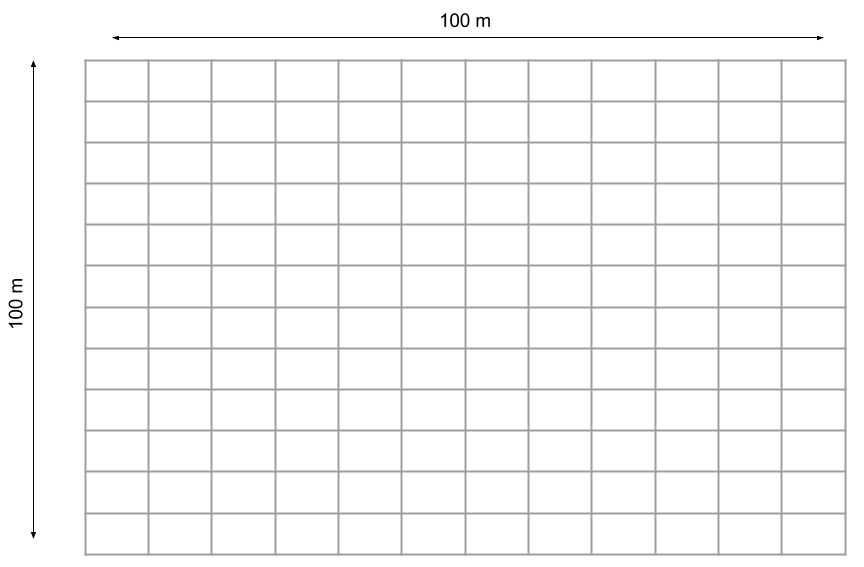
\includegraphics[width=\textwidth/2]{simulation_grid.png}
	\caption{ Gridded simulation area.}	
	\label{fig:simulation_grid}
\end{figure}

The size of individual cells can be configured to increase/decrease the resolution and, therefore, the accuracy of the simulation. As the simulation progresses, plant's grow, their spatial coverage increases, and they enter new grid cells. When a plant enters a new grid cell, it becomes a member of it and cell resources must be distributed to it as well as to all other plants in the cell. The information associated to each individual grid cell can be split into two categories: \textit{time-dependent} and \textit{simulation-dependent}. The time-dependent information depends only on the current month, is identical for every grid cell and is comprised of: the \textit{soil humidity} and the \textit{illumination}. The simulation-dependent information changes throughout the simulation as plants spawn, die and grow and is comprised of: the list of plants whose roots intersect the cell and the list of plants whose canopy intersects the cell.

\subsection{Resource Distribution}

The strength of each plant in the simulation must be recalculated on a monthly basis. To determine the strength of a given plant, it is necessary to know the illumination and humidity allocated to it along with the temperature. The temperature is not a distributable resource and is identical for all plant instances given the month. The allocated humidity and illumination is determined by averaging the resources distributed to it in each cell it overlaps in the grid. So, before the strengths of individual plant instances can be calculated, first each cell of the grid must be iterated over and illumination and humidity distributed to the plants contained within. How these are allocated is discussed below.

\subsubsection{Humidity Distribution}

Plants grow there roots in order to access the nutrients and moisture available in the surrounding soil. As roots of different plants overlap, they start to compete for these resources.\\

When distributing the soil humidity of a given grid cell \textit{C$_{xy}$} to the set \textit{S} = \{P$_{1}$, P$_{2}$, P$_{3}$, ...\} of plants which roots intersect the cell, one of three distinct scenarios can occur depending on the total available humidity of the cell: \textit{Abundant humidity}, \textit{sufficient humidity} and \textit{insufficient humidity}.\\

The humidity is deemed abundant if the available humidity, \textit{H$_{available}$}, surpasses 300 millimetres. In this situation, the humidity is deemed to be enough for there to be standing water and therefore all plants of \textit{S} are allocated \textit{H$_{available}$}. \\

If \textit{H$_{available}$} is less than 300 millimetres, it is necessary to determine whether the humidity is sufficient or insufficient by calculating the requested humidity \textit{H$_{requested}$} as outlined in equation \ref{eq:humidity_requested_calc}. 

\begin{equation}
H_{requested} = \sum MinHumidity(P_{n}) \text{ for } n \in S
\label{eq:humidity_requested_calc}
\end{equation}
Where:\textit{MinHumidity(P$_{n}$)} is the minimum humidity requirement of the specie to which plant \textit{P$_{n}$} belongs;\textit{S} is the set of plants whose roots intersect with the given grid cell.

If \textit{H$_{requested}$} is less than \textit{H$_{available}$}, the humidity is deemed sufficient and the amount allocated to each plant is calculated as described in equation \ref{eq:humidity_allocation_sufficient_calc}. If \textit{H$_{requested}$} is more than \textit{H$_{available}$}, however, the humidity is deemed insufficient and the allocation is done following equation \ref{eq:humidity_allocation_insufficient_calc}

\begin{equation}
\begin{split}
H_{allocated}(P_{n}) = MinHumidity(P_{n}) + OverFlow \\
OverFlow = H_{available} - \sum MinHumidity(P_{n}) \text{ for } n \in S
\end{split}
\label{eq:humidity_allocation_sufficient_calc}
\end{equation}
Where:\textit{H$_{allocated}$(P$_{n}$)} is the humidity allocated to plant \textit{P$_{n}$}; \textit{MinHumidity(P$_{n}$)} is the minimum humidity requirement of the specie to which plant \textit{P$_{n}$} belongs;\textit{S} is the set of plants whose roots intersect with the given grid cell.

Intuitively, it allocates each plant with the minimum amount of humidity it requires to survive plus the resulting overflow.

\begin{equation}
\begin{split}
H_{allocated}(P_{n}) = min(MinHumidity(P_{n}), Vigor(P_{n}) \times H_{remaining}) \\
Vigour(P_{n}) =  \frac{RootSize(P_{n})}{\sum RootSize(P_{x}) \text{ for } x \in S}\\
H_{remaining} = H_{available} - (\sum H_{allocated}(P_{x})  \text{ for } x \in S_{processed})\\
\end{split}
\label{eq:humidity_allocation_insufficient_calc}
\end{equation}
Where: The plants of \textit{S} \textbf{must} be iterated over in decrementing order of their vigor as this will affect the water they are allocated; \textit{H$_{allocated}$(P$_{n}$)} is the humidity allocated to plant \textit{P$_{n}$}; \textit{MinHumidity(P$_{n}$)} is the minimum humidity requirement of the specie to which plant \textit{P$_{n}$} belongs; \textit{Vigour(P$_{n}$)} is the vigor of plant \textit{P$_{n}$} in comparison to other plants present in the cell. It is estimated based on root size; \textit{RootSize(P$_{n}$)} is the root size of plant \textit{P$_{n}$}; S$_{processed}$) is the set of plants from \textit{S} whose water allocation has already been calculated; \textit{S} is the set of plants whose roots intersect with the given grid cell.

Intuitively, this algorithm prioritises water distribution to more vigorous plant's.

\subsubsection{Plant Humidity Allocation}

To calculate the humidity allocated to plant \textit{P$_{n}$}, it is first necessary to determine the set of grid cells \textit{S} = \{C$_{1}$, C$_{2}$, C$_{3}$, ...\} which it's roots intersect. Given this, the plants humidity allocation is calculated using equation \ref{eq:plant_humidity_allocation}. 

\begin{equation}
H_{n} = \frac{\sum H_{allocated}(C_{x}) \text{ for } x \in S}{| S |}
\label{eq:plant_humidity_allocation}
\end{equation}
Where:\textit{H$_{n}$} is the humidity allocated to plant \textit{P$_{n}$}; \textit{H$_{allocated}$(C$_{n}$)} is the humidity allocated to plant \textit{P$_{n}$} in grid cell C$_{n}$; \textit{$|$ S $|$} is the number of cells in the set \textit{S}.

Intuitively, the humidity allocated to a given plant is simply the average of the humidity allocated to it in all grid cells it's roots intersect.

\subsubsection{Illumination Distribution}

Plants which are heavily dependent on illumination will often grow a large canopy in order to maximize the leaf area receiving direct sunlight. Doing so also restricts the illumination received by smaller plants in the undergrowth. To model the shade projection of larger plants, illumination is distributed in each cell depending on the plants height and canopy width.\\

Equation \ref{eq:illum_distribution} is used to allocate illumination amongst the set \textit{S} = \{P$_{1}$, P$_{2}$, P$_{3}$, ...\} of plants which canopy intersects cell \textit{C$_{xy}$}.

\begin{equation}
\centering
Illumination(P_{n}) = 
\begin{cases}
	C_{illumination}, & \text{if } CanopyWidth(P_{n}) = 0 for x \in S \\
	C_{illumination}, & \text{if } Height(P_{n}) > height(x) for x \in S : x \neq P_{n} \\
    0,              & \text{otherwise}
\end{cases}
\label{eq:illum_distribution}
\end{equation}
Where: \textit{Illumination($P_{n}$)} is the illumination allocated to plant \textit{P$_{n}$} whose canopy overlaps with current grid cell;\textit{C$_{illumination}$} is the monthly illumination of the cell;\textit{CanopyWidth(P$_{n}$)} is the canopy width of plant P$_{n}$; \textit{Height(P$_{n}$)} is the height of plant P$_{n}$; \textit{S} is the set of plants whose canopy intersects with the given grid cell.

Intuitively, if all plants present in the given cell are canopy-free (i.e no shade projection), the equation allocates them all the available illumination. If not all plants are canopy-free, the equation allocates illumination only to the tallest canopy plant.

\subsubsection{Plant Illumination Allocation}

Calculating the illumination allocated to a plant \textit{P$_{n}$} is very similar to calculating the humidity allocation only the set of grid cells \textit{S} = \{C$_{1}$, C$_{2}$, C$_{3}$, ...\} are those which the plants canopy intersects. Given \textit{S}, the plant illumination is calculated using equation \ref{eq:plant_illumination_allocation}.

\begin{equation}
I_{n} = \frac{\sum I_{allocated}(C_{x}) \text{ for } x \in S}{| S |}
\label{eq:plant_illumination_allocation}
\end{equation}
Where:\textit{I$_{n}$} is the illumination allocated to plant \textit{P$_{n}$}; \textit{I$_{allocated}$(C$_{n}$)} is the illumination allocated to plant \textit{P$_{n}$} in grid cell C$_{n}$; \textit{$|$ S $|$ } is the number of cells in the set \textit{S}.

Intuitively, the illumination allocated to a given plant is simply the average of the humidity allocated to it in all grid cells it's canopy intersect.

\subsection{Plant Strength Calculation}

The strength of plant \textit{P$_{n}$} is the minimum of \textit{S$_{age}$}, \textit{S$_{temperature}$}, \textit{S$_{illumination}$} and \textit{S$_{humidity}$} which represent the strength of the plant in terms of it's age, temperature, illumination and humidity respectively. To calculate these values, ranging from negative to positive one hundred, a graph is plotted for each specie based on it's properties as outlined in figures \ref{fig:strength_calc_age}, \ref{fig:strength_calc_temp}, \ref{fig:strength_calc_temp}, \ref{fig:illumination_strength} and \ref{fig:humidity_strength}. Using these graphs, it is possible to calculate the strength of any plant given it's allocated resources.

\begin{figure}
\center
	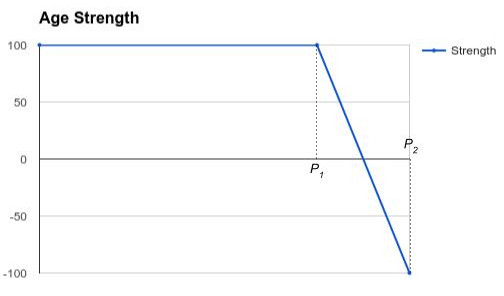
\includegraphics[scale=0.7]{age_strength.jpg}
	\caption{ Graph used to calculate the age strength of any plant. \textbf{P$_{1}$} is the age of \textit{start of decline} configured for the given specie. \textbf{P$_{2}$} is the \textit{maximum age} configured for the given specie. }	
	\label{fig:strength_calc_age}
\end{figure}

\begin{figure}
\center
	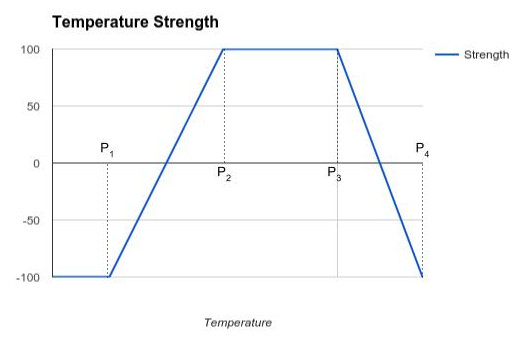
\includegraphics[scale=0.7]{temperature_strength.jpg}
	\caption{ Graph used to calculate the temperature strength of any plant. \textbf{P$_{1}$} and \textbf{P$_{4}$} are the \textit{minimum} and \textit{maximum temperature} configured for the given specie. \textbf{P$_{2}$} and \textbf{P$_{3}$} form the \textit{prime temperature range} configured for the given specie.  }	
	\label{fig:strength_calc_temp}
\end{figure}

\begin{figure}
\center
	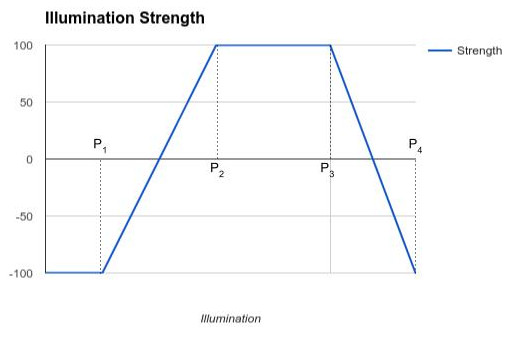
\includegraphics[scale=0.7]{illumination_strength.jpg}
	\caption{ Graph used to calculate the illumination strength of any plant. \textbf{P$_{1}$} and \textbf{P$_{4}$} are the \textit{minimum} and \textit{maximum illumination} configured for the given specie. \textbf{P$_{2}$} and \textbf{P$_{3}$} form the \textit{prime illumination range} configured for the given specie.  }	
	\label{fig:illumination_strength}
\end{figure}

\begin{figure}
\center
	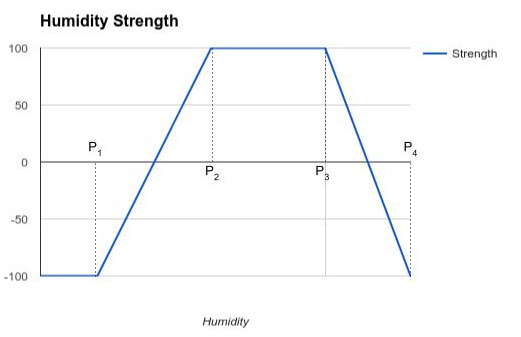
\includegraphics[scale=0.7]{humidity_strength.jpg}
	\caption{ Graph used to calculate the humidity strength of any plant. \textbf{P$_{1}$} and \textbf{P$_{4}$} are the \textit{minimum} and \textit{maximum humidity} configured for the given specie. \textbf{P$_{2}$} and \textbf{P$_{3}$} form the \textit{prime humidity range} configured for the given specie.  }	
	\label{fig:humidity_strength}
\end{figure}

\subsection{Plant Strength Usage}

The strength of each plant is recalculated on a monthly basis as available resources change and other plants spawn and grow. This value subsequently influences its growth potential and probability of death, as discussed below.

\subsubsection{Growth Potential}

In the simulation, each plant \textit{P} attempts to grow its roots, its canopy and it's height on a monthly basis. Each specie has an maximum monthly root growth \textit{MaxGrowth$_{root}$}, canopy growth \textit{MaxGrowth$_{canopy}$} and height growth \textit{MaxGrowth$_{height}$} which are calculated using the specie's growth and ageing properties as outlined in equations \ref{eq:max_root_growth}, \ref{eq:max_canopy_growth} and \ref{eq:max_height_growth} respectively.

\begin{equation}
MaxGrowth_{root}(S) = \frac{MaxRoot(S)}{Age_{StartOfDecline}(S)}
\label{eq:max_root_growth}
\end{equation}
Where:\textit{MaxGrowth$_{root}$(S)} is the maximum monthly root growth of specie \textit{S};\textit{MaxRoot(S)} is the configured maximum root size of the specie \textit{S};\textit{Age$_{StartOfDecline}$(S)} is the age of start of decline configured for specie \textit{S}.

\begin{equation}
MaxGrowth_{canopy}(S) = \frac{MaxCanopy(S)}{Age_{StartOfDecline}(S)}
\label{eq:max_canopy_growth}
\end{equation}
Where:\textit{MaxGrowth$_{canopy}$(S)} is the maximum monthly canopy growth of specie \textit{S};\textit{MaxCanopy(S)} is the configured maximum canopy size of specie \textit{S};\textit{Age$_{StartOfDecline}$(S)} is the age of start of decline configured for specie \textit{S}.

\begin{equation}
MaxGrowth_{height}(S) = \frac{MaxHeight(S)}{Age_{StartOfDecline}(S)}
\label{eq:max_height_growth}
\end{equation}
Where:\textit{MaxGrowth$_{height}$(S)} is the maximum monthly height growth of specie \textit{S};\textit{MaxHeight(S)} is the configured maximum height of specie \textit{S};\textit{Age$_{StartOfDecline}$(S)} is the age of start of decline configured for specie \textit{S}.

The actual root growth \textit{Growth$_{root}$}, canopy growth \textit{Growth$_{canopy}$} and height growth \textit{Growth$_{height}$} is directly dependent on the plant's strength, however, and is calculated using equations \ref{eq:actual_root_growth}, \ref{eq:actual_canopy_growth} and \ref{eq:actual_height_growth} respectively. The maximum growth is achieved only if the plant is at its full strength. Note that no plants grow if there current strength is negative as they are deemed in a \textit{survival state}.

\begin{equation}
Growth_{root}(\textit{P},S) = max(0, Strength(\textit{P}) \times  MaxGrowth_{root}(S)
\label{eq:actual_root_growth}
\end{equation}
Where:\textit{Growth$_{root}$(S)} is the monthly root growth of plant \textit{P} of specie \textit{S};\textit{Strength(\textit{P}} is the current strength of \textit{P};\textit{MaxGrowth$_{root}$(S)} is the maximum monthly root growth calculated for specie \textit{S}.

\begin{equation}
Growth_{canopy}(\textit{P},S) = max(0, Strength(\textit{P}) \times  MaxGrowth_{canopy}(S)
\label{eq:actual_canopy_growth}
\end{equation}
Where:\textit{Growth$_{canopy}$(S)} is the monthly canopy growth of plant \textit{P} of specie \textit{S};\textit{Strength(\textit{P}} is the current strength of \textit{P};\textit{MaxGrowth$_{canopy}$(S)} is the maximum monthly canopy growth calculated for specie \textit{S}.

\begin{equation}
Growth_{height}(\textit{P},S) = max(0, Strength(\textit{P}) \times  MaxGrowth_{height}(S)
\label{eq:actual_height_growth}
\end{equation}
Where:\textit{Growth$_{height}$(S)} is the monthly height growth of plant \textit{P} of specie \textit{S};\textit{Strength(\textit{P}} is the current strength of \textit{P}; \textit{MaxGrowth$_{height}$(S)} is the maximum monthly height growth calculated for specie \textit{S}.

\subsubsection{Probability of Death}

On a monthly basis, the probability of death of each plant is calculated based on it's strength using equation \ref{eq:probability_of_death} and the plant killed with the said probability. Note that a plant \textit{P} will only be susceptible to be killed off if it's strength is negative. 

\begin{equation}
Probability_{death}(P) = max(0, \frac{-1 \times Strength(P) + counter}{100})
\label{eq:probability_of_death}
\end{equation}
Where:\textit{Probability{death}(P)} is the probability of death of plant \textit{P};\textit{Strength(\textit{P}} is the current strength of \textit{P};\textit{counter} is a value which increases by ten each month the plant's strength is negative and resets to zero when it becomes positive. This is to prevent plant's from surviving with a continuous negative strength for too long.

\subsection{Spawning Plants}

In nature, the spawning of new plants ensures specie \textit{succession} and \textit{propagation}. In order to accurately model the evolution of an ecosystem it is essential to replicate this spawning mechanism. To do so, seeds are produced annually for each specie and are positioned either randomly or at predefined positions. The number of seeds that are produced for a given specie is determined by the specie's \textit{annual seed count} configuration.\\

Different seeding mechanisms are used in the simulator depending on the number of plant's of the given specie present in the simulation, \textit{S$_{count}$}, and it's illumination properties.\\
If \textit{S$_{count}$} is greater than zero, existing plant instances are used to determine the location of new plants, irrespective of it's illumination requirements, as described in \textit{Spawning from Existing Plants}.\\
If \textit{S$_{count}$} is zero, the seeding mechanism depends on the specie's illumination requirements. If the specie is shade loving, \textit{canopy seeding} is employed, else \textit{random seeding}. Both are discussed below.

\subsubsection{Spawning from Existing Plants}

To ensure specie propagation, when plant's of the given specie are already present in the simulation window, they are used to determine the location for new plant instances. To do so, \textit{n} of these plants are selected at random and seeds placed at random within an annular radius \textit{r} of each. The value of \textit{n} is the \textit{annual seed count} configured for the current specie. The value of \textit{r} is the configured \textit{maximum seeding distance} of the specie. Note that if the number of plants of the given specie is less than the number of seeds to produce, a single plant is used to produce multiple seed locations. \\

This technique effectively ensures \textit{propagation} until the number of plant instances present is larger than the number of seeds to produce. At which point, the \textit{propagation} potential decreases as the plant count increases. This is because as the selection pool for the random plants increases in size, the probability of selecting a plant at a location which will permit propagation decreases. To overcome this and ensure the initial seeding plants that are selected span a wide area of the simulation window, they are selected at from individual simulation grid cells.\\

\subsubsection{Canopy Seeding}

Shade-loving plants strive in the shaded undergrowth. If shade-loving plants are spawned at random locations in the simulation, the probability of them landing under the canopy of an existing plant is extremely low. To overcome this, shade-loving plants are not spawned at random but under the canopy of randomly selected plants.

\subsubsection{Random Seeding}

This is the most simple form of seeding and is used when no plants of the given specie are present in the simulation and the specie is not shade-loving. The set of locations for new plants to spawn is selected at random within the simulation window.

\subsection{Performance} \label{subsec:ecosytem_performance}

The number of plants present in the simulation will heavily influence it's performance as the strength of each plant needs to be recalculated on a monthly basis. To test the influence of plant count on simulation time, a simulation is run with a single specie of plant and the monthly processing time analysed alongside the number of plants present. The plant used is grass at is has no canopy and very minimal root coverage, permitting a large number of instances to grow simultaneously (see appendix \ref{AppendixB} for properties of specie). The resources were set to be optimal for maximizing plant count and minimizing intra-plant competition. The simulation is started with only a single instance and, as the simulation progresses and seeding is performed, the number of instances increase. The results are summarized in Figure \ref{fig:ecosimulator_test_plant_count} and show that the processing time increases linearly with plant count. \\

\begin{figure}
\center
	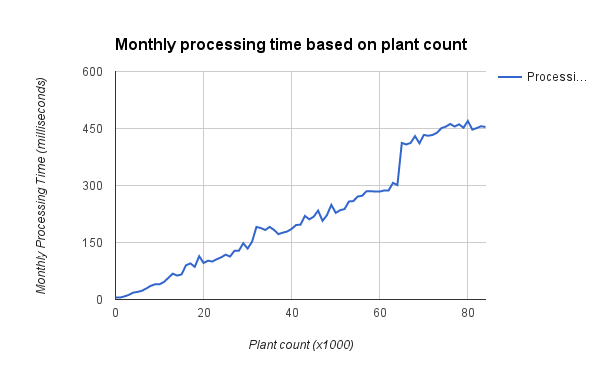
\includegraphics[scale=0.7]{ecosimulator_test_plant_count.png}
	\caption{ Processing time based on plant count. Total simulation time for 100 years: 271 seconds}	
	\label{fig:ecosimulator_test_plant_count}
\end{figure}

Another simulation property which heavily impacts performance is the root and canopy growth of plant species present. The reason for this is that, as plant's roots and canopy grow, they will cover more simulation grid cells and more calculations will be required per individual cell when the contained resources are distributed. To analyse the impact of plant growth, a base specie \textit{S$_{base}$} is created with a given root and canopy growth rate. Then, two species are created \textit{S$_{X2}$} and \textit{S$_{X3}$} with twice and thrice the growth rates of \textit{S$_{base}$} respectively (see appendix \ref{AppendixB} for specie details). An identical simulation is run on each specie in terms of available resources and, on a monthly basis, the number of plants present in the simulation along with the monthly processing time analysed. Given this information, it is possible to track the average monthly processing time per plant throughout the simulation. It is important to normalise based on the number of plants as the faster growing plants will permit less plants to survive for the simple reason that they will require and be able to access resources from a larger amount of grid cells. As can be seen in the results plotted in figure \ref{fig:ecosimulator_test_per_plant}, the processing times are similar to start and then increase proportionally to the species growth rate.

\begin{figure}
\center
	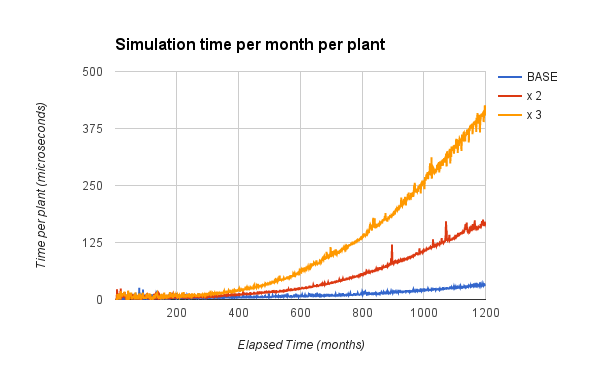
\includegraphics[scale=0.7]{ecosimulator_test_per_plant.png}
	\caption{ Evolution of the monthly processing time normalised based on plant count. The processing time increases as the plant's grow larger as they cover more grid cells. Total simulation time for one hundred years: ~49 seconds for \textit{S$_{base}$}, ~122 seconds for \textit{S$_{X2}$} and 166 seconds for \textit{S$_{X3}$}}
	\label{fig:ecosimulator_test_per_plant}
\end{figure}

\subsection{Results}

To test the resulting spatial distribution of plant communities in their work, Lane and and Przemyslaw \cite{Lane2002} attempt to reproduce three important properties of nature: \textit{Self-thinning}, \textit{succession} and \textit{propagation}.\\
As plants grow, their resource requirements increase and, as a direct consequence, inter-plant competition for resources increases. Eventually, the competition becomes too intense and resources too scarce leading to more vigorous plants starving smaller plants. At this point, \textit{self-thinning} begins and plant densities decrease.\\
Given plant specie A with a fast growth rate and specie B with a slower growth rate but higher shade tolerance. At first, the faster growing specie A will dominate and flourish but, with time, the slower growing but more shade tolerant specie B will flourish and dominate. This is the \textit{succession} property.\\
Plants \textit{propagate} in clusters surrounding the seeding plant.\\

To test the ecosystem simulator, we will first employ the same methodology as Lane and and Przemyslaw \cite{Lane2002} and attempt to reproduce \textit{self-thinning}, \textit{succession} and \textit{propagation}.

To ensure a given plant specie strives better in its optimal environment, the same simulation will be run using a single plant specie with varying resource properties and the resulting plant distribution analysed. This test is discussed in \textit{Varying Resources Test} below.\\

A \textit{shade-simulation test} is performed to ensure plants which depend on direct illumination strive less in the shaded undergrowth of larger plants.\\ 

To ensure shade-loving plants are able to propagate and strive under the canopies of larger plants, a \textit{shade-loving plant test} is also performed.

\subsubsection{Self-thinning Test}

\textit{Self-thinning} occurs when the plant biomass surpasses a given tipping point where available resources become insufficient to permit further plant growth. At this point, larger plants start to kill off smaller, weaker plants by stealing their resources.\\

To test whether self-thinning is successfully modelled in the ecosystem simulator, three simulations are run as described in table \ref{tab:self_thinning_test_simulations} and the plant count tracked throughout. As described previously, self-thinning occurs because of insufficient resources. By modifying only available humidity in each simulation, it's effect on self-thinning becomes apparent. As can be seen in the results summarized in figure \ref{fig:self_thinning_test_results}, the plant count increases at first, reaches a maximum and decreases thereafter. This is the exact behaviour of self-thinning. Furthermore, it is apparent that the maximum plant count increases with the humidity available, therefore showing that self-thinning is sensitive to available resources.

\begin{table}[]
  \centering
	    \begin{tabular}{|p{3cm}|p{3cm}|p{3cm}|p{3cm}|p{3cm}|}
		\hline
		\textbf{Simulation} & \textbf{Simulation time (years)} & \textbf{Humidity} & \textbf{Illumination} & \textbf{Temperature}\\
		\hline       
		1 & 100 & 25 & 10 & 15\\           
		\hline       
		2 & 100 & 30 & 10 & 15\\   
		\hline       
		3 & 100 & 35 & 10 & 15\\              
		\hline       
		\end{tabular}
		\caption{Self-thinning test simulation configurations. For simplicity, monthly resources are kept constant.}
		\label{tab:self_thinning_test_simulations}
\end{table}

\begin{figure}
\center
	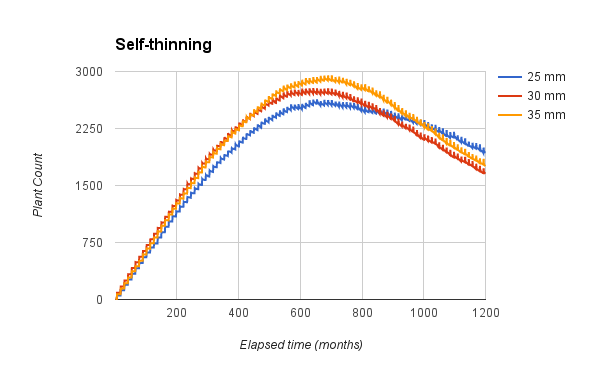
\includegraphics[scale=0.7]{self_thinning.png}
	\caption{ Plant count tracked throughout three separate simulations differing only in available humidity. }
	\label{fig:self_thinning_test_results}
\end{figure}

\subsubsection{Succession Test}

Succession occurs in an ecosystem due to the different growth rates of the species it contains. To test \textit{succession} in the ecosystem simulator, two plant species \textit{S$_{fast}$} and \textit{S$_{slow}$} are created differing only in their growth rate and illumination properties (see appendix \ref{AppendixB} for details) and a simulation run with these two species under optimal conditions. During the simulation, the appearance and average size of the two plant species are monitored to determine the dominating specie. The analytical results illustrated in figure \ref{fig:succession_plants_avg_size} along with the appearance at ten year intervals displayed in figure \ref{fig:succession_plants_render} shows that \textit{S$_{fast}$} dominates at first (~300 months in) followed by \textit{S$_{slow}$} (~500 months in). A balance is found thereafter.

\begin{figure}
\center
	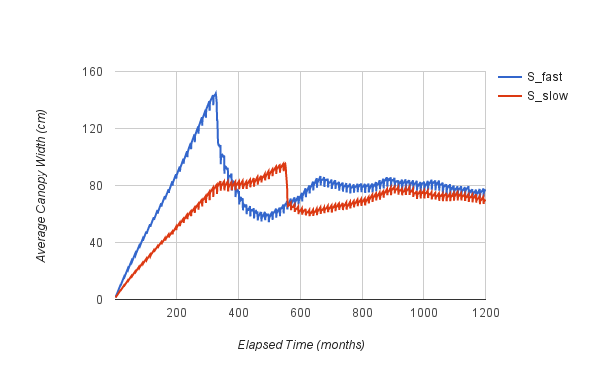
\includegraphics[scale=0.7]{succession_plant_avg_size.png}
	\caption{ Succession Test: Average size of the slow growing S$_{slow}$ (red) and fast growing S$_{fast}$ (blue) throughout a simulation run in optimal conditions. }
	\label{fig:succession_plants_avg_size}
\end{figure}

\begin{figure}
\center
	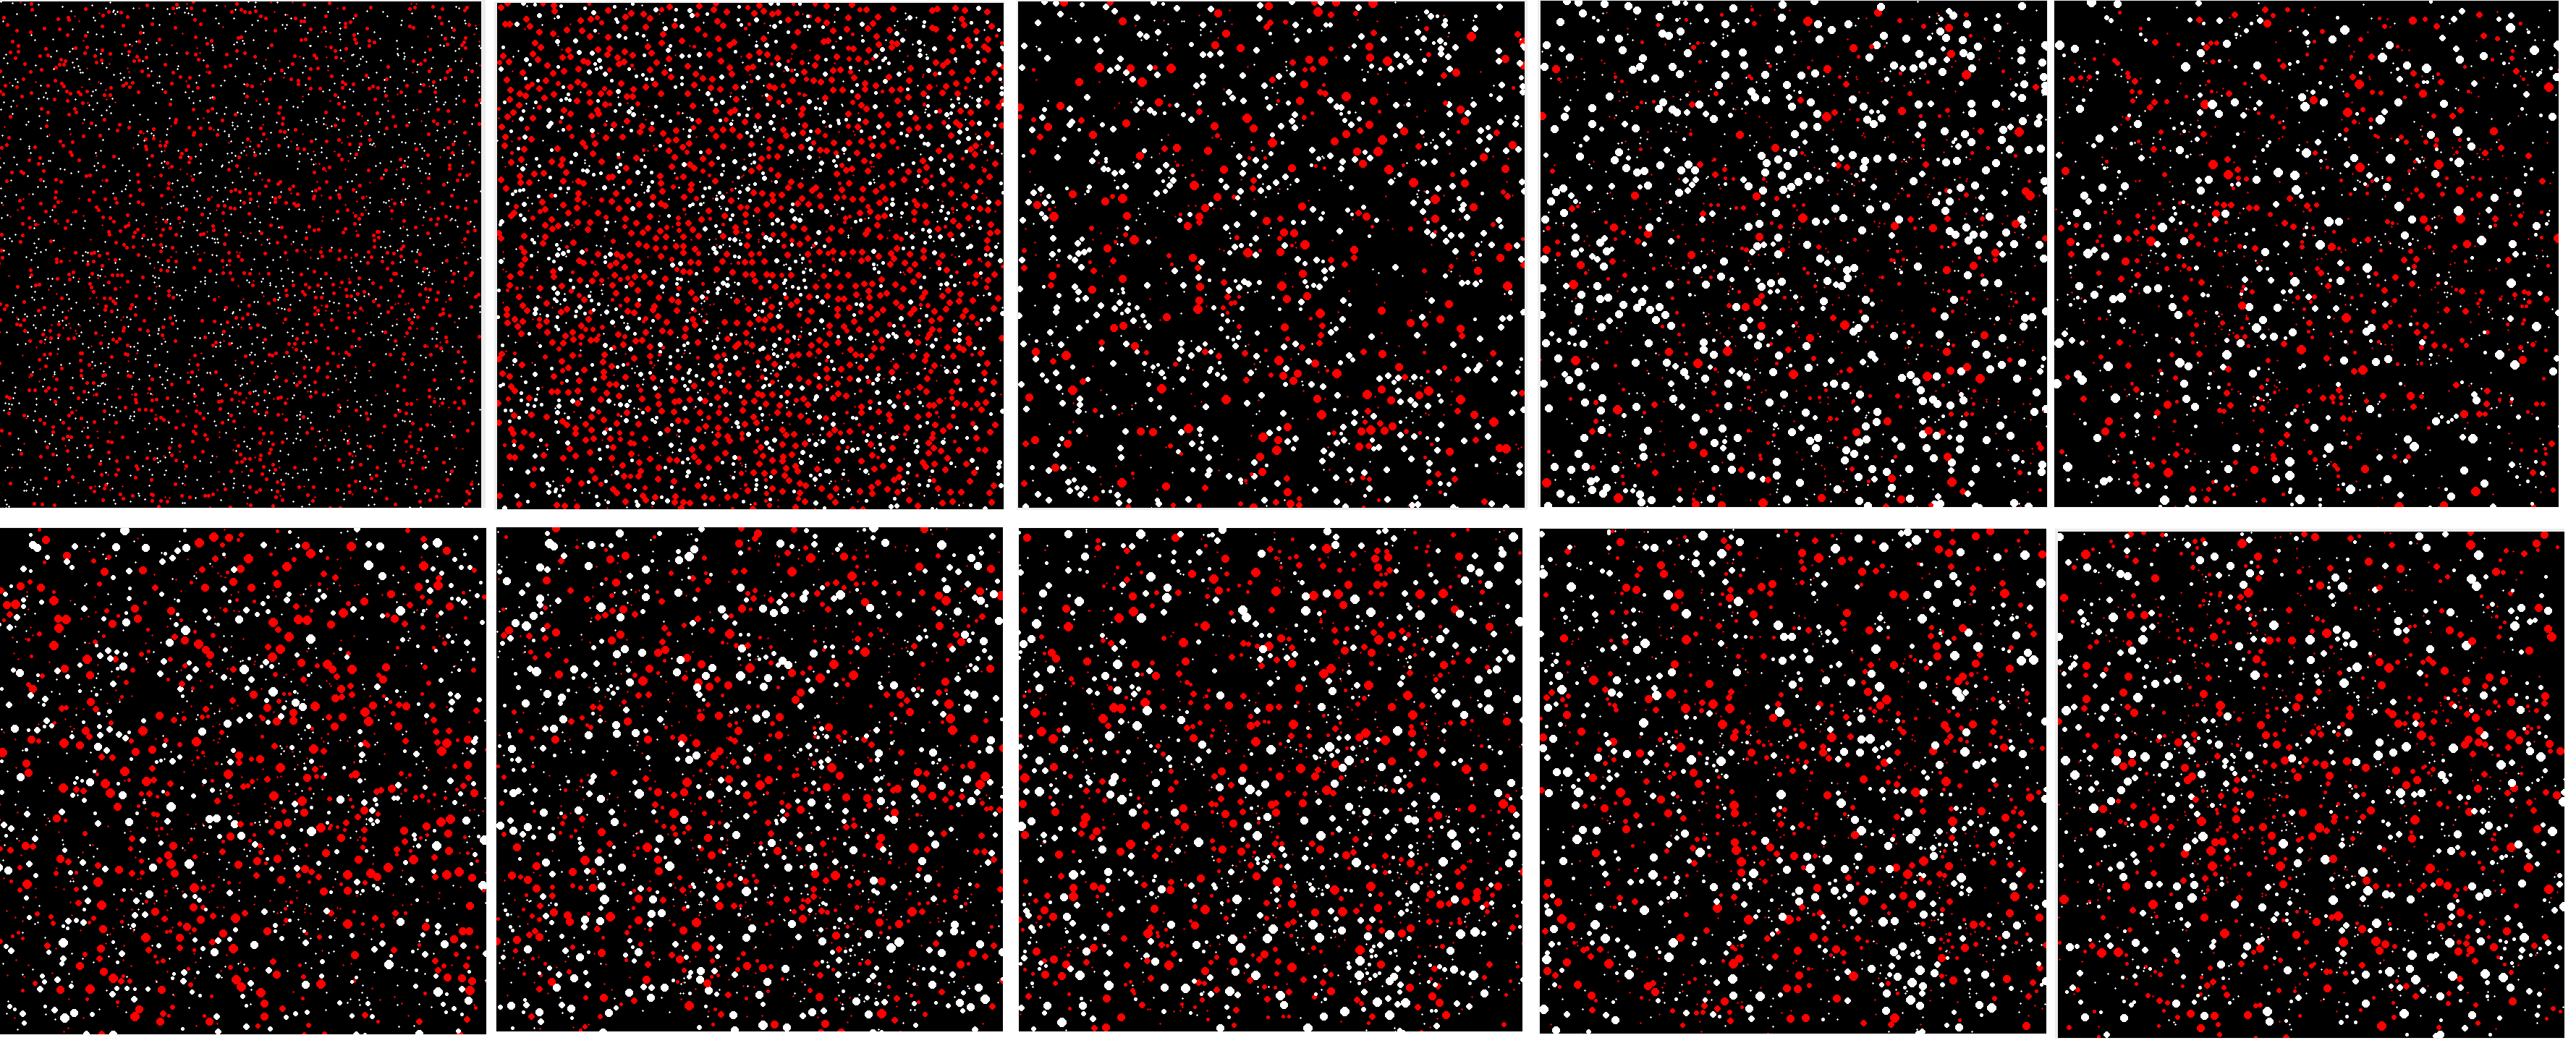
\includegraphics[width=\textwidth]{succession_plants_render.png}
	\caption{ Succession Test: Appearance of the slow growing S$_{slow}$ (white) and fast growing S$_{red}$ (blue) at different times during the simulation. From left-to-right, top-top-bottom: 10, 20, 30, 40, 50, 60, 70, 80, 90 and 100 years.}
	\label{fig:succession_plants_render}
\end{figure}

\subsubsection{Propagation Test}

To ensure propagation is modelled in the ecosystem simulator a simulation is run with a single starting grass seed (see appendix \ref{AppendixB} for specie details) and it's evolution tracked throughout. Figure \ref{fig:propagation_test_render} shows that iterative propagation through annual seeding enables a single seed plant to colonize the entirety of the terrain. 

\begin{figure}
\center
	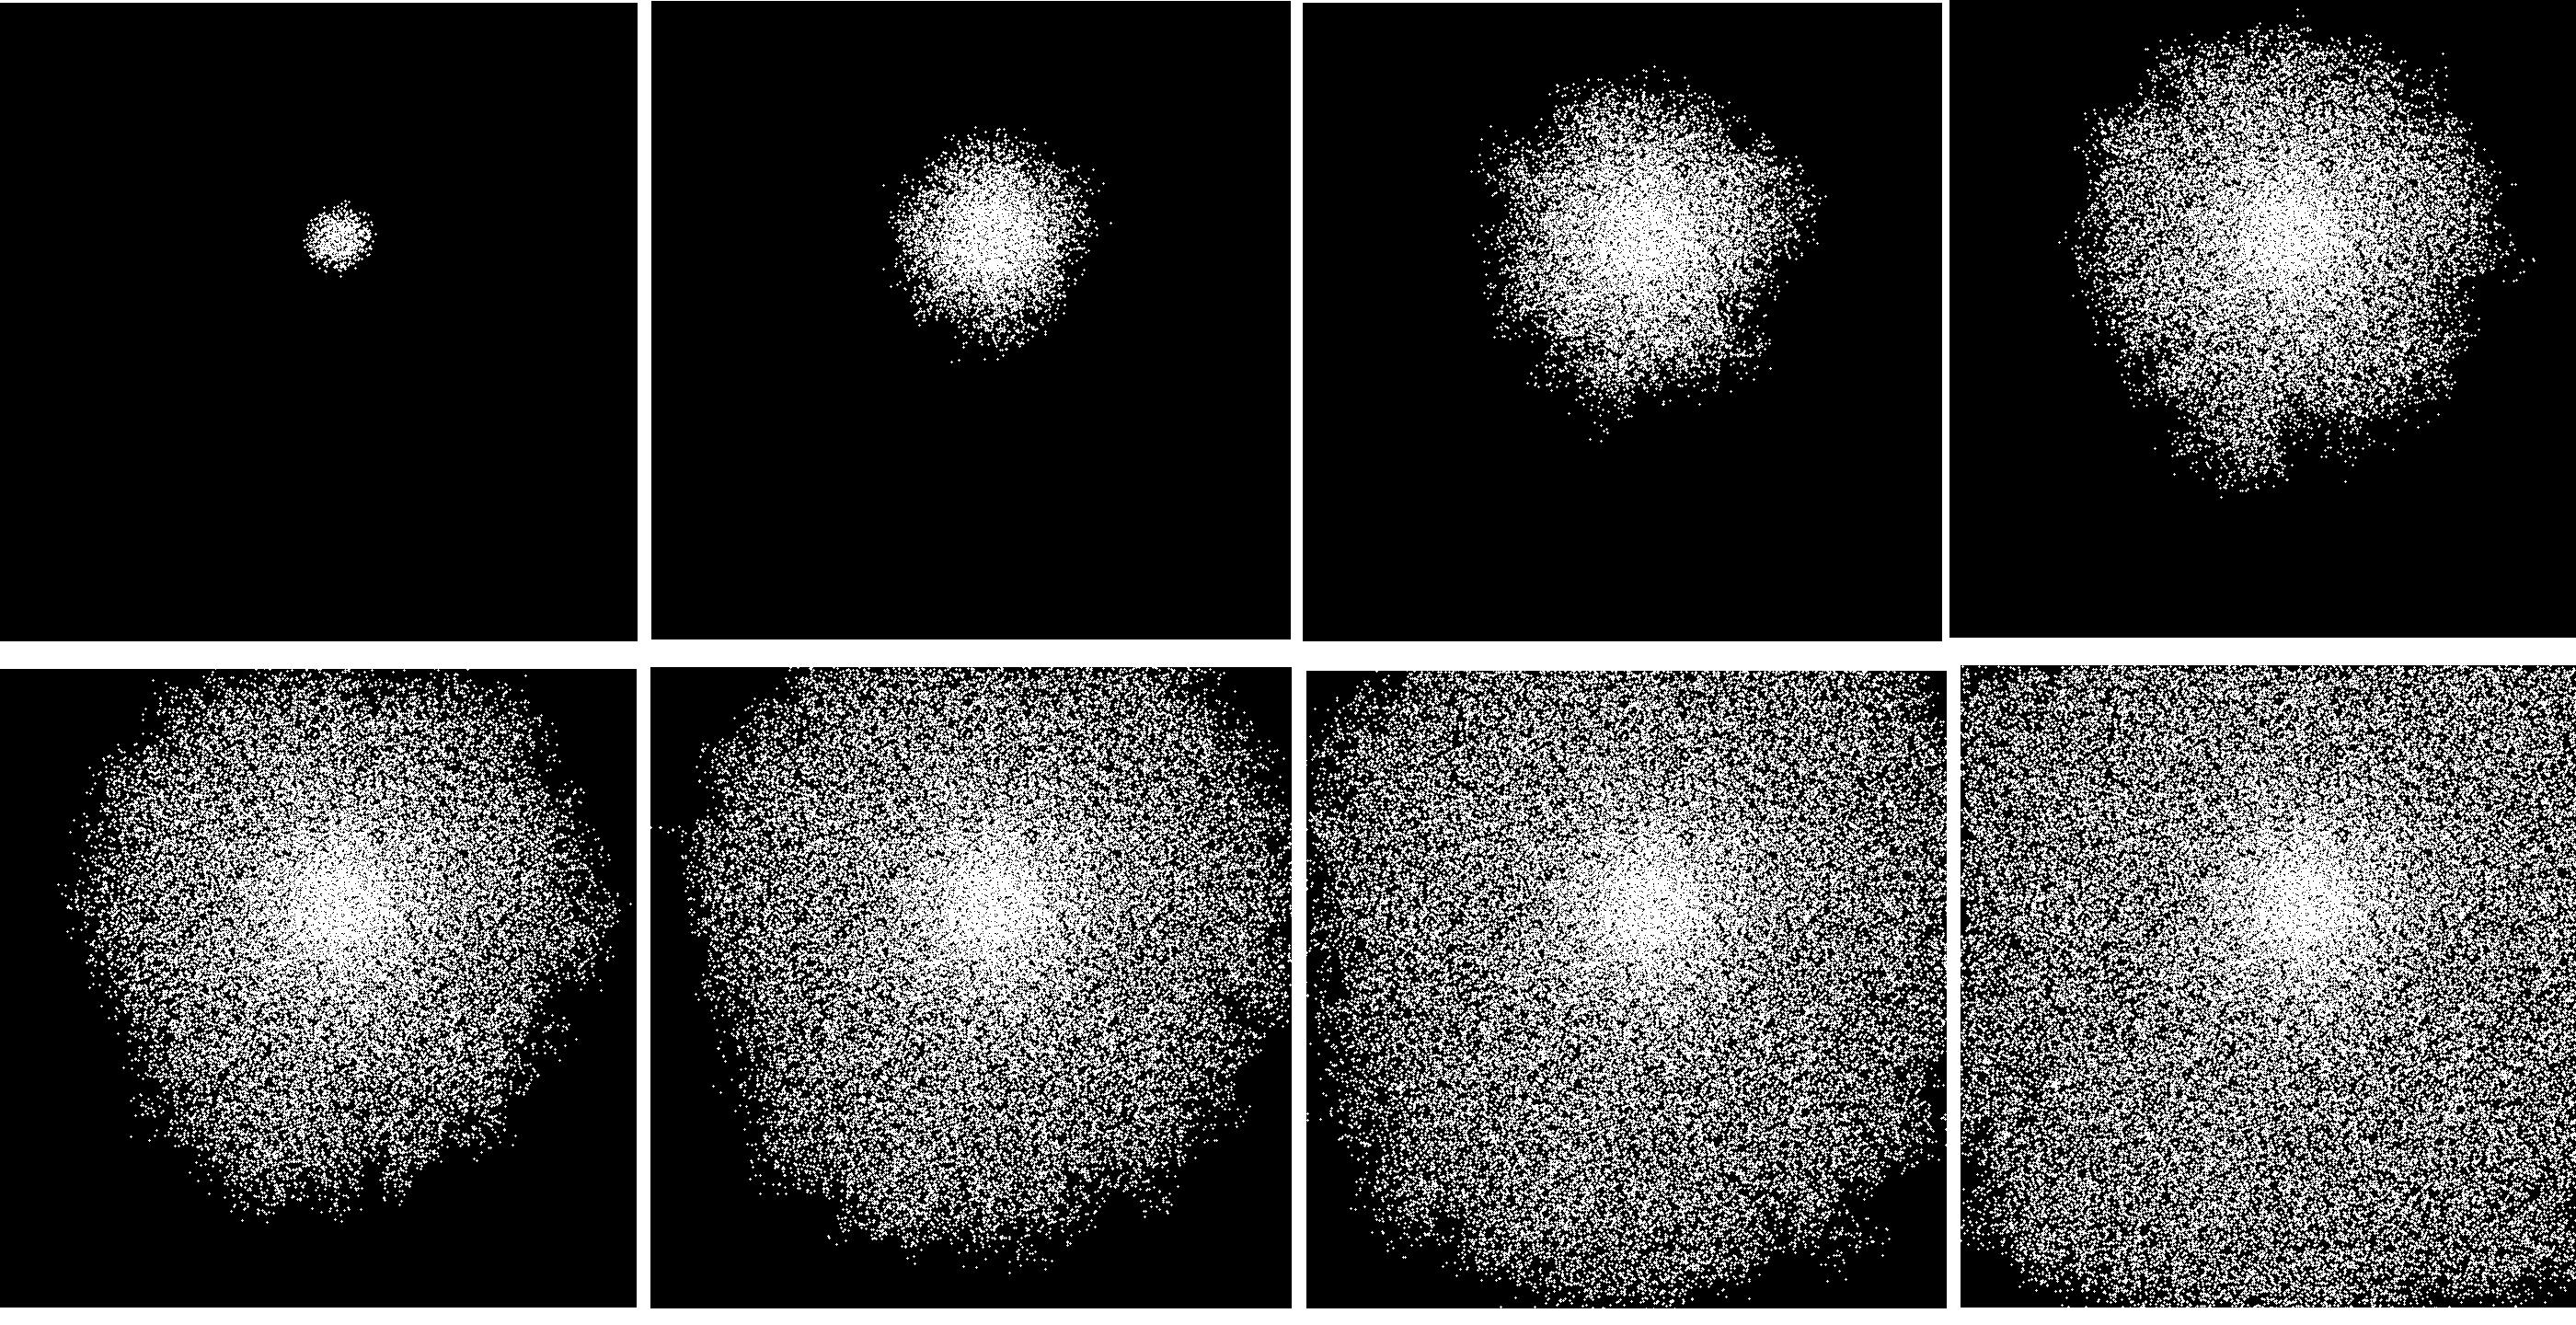
\includegraphics[width=\textwidth]{propagation_test_render.png}
	\caption{ Propagation Test: Evolution through time of a simulation starting from a single seed plant of grass. From left-to-right, top-to-bottom: 2, 10, 20, 30, 40, 50, 60, 70 years in.}
	\label{fig:propagation_test_render}
\end{figure}

\subsubsection{Varying Resource Test}

To ensure a given plant specie strives better when it's habitat is more suited, multiple simulations are run with only specie \textit{S$_{base}$} (see appendix \ref{AppendixB} for specie properties) present. As outlined in table \ref{tab:varying_resource_test_simulations}, the simulations vary only in their configured humidity. As seen by the results plotted in figure \ref{fig:varying_resource_test}, illustrating the average canopy width for a single plant instance throughout the simulations, plants strive better in environments better suited to their resource requirements.

\begin{table}[]
  \centering
	    \begin{tabular}{|p{3cm}|p{3cm}|p{3cm}|p{3cm}|p{3cm}|}
		\hline
		\textbf{Simulation} & \textbf{Simulation time (years)} & \textbf{Humidity} & \textbf{Illumination} & \textbf{Temperature}\\
		\hline         
		1 & 100 & 22 & 10 & 20\\           
		\hline       
		2 & 100 & 24 & 10 & 20\\
		\hline       
		3 & 100 & 26 & 10 & 20\\           
		\hline     
		4 & 100 & 28 & 10 & 20\\           
		\hline     
		5 & 100 & 30 & 10 & 20\\           
		\hline       
		6 & 100 & 32 & 10 & 20\\           
		\hline       
		7 & 100 & 34 & 10 & 20\\           
		\hline      
		8 & 100 & 36 & 10 & 20\\           
		\hline       
		9 & 100 & 38 & 10 & 20\\           
		\hline     
		\end{tabular}
		\caption{Varying resource rest simulation configurations. For simplicity, monthly resources are kept constant.}
		\label{tab:varying_resource_test_simulations}
\end{table}

\begin{figure}
\center
	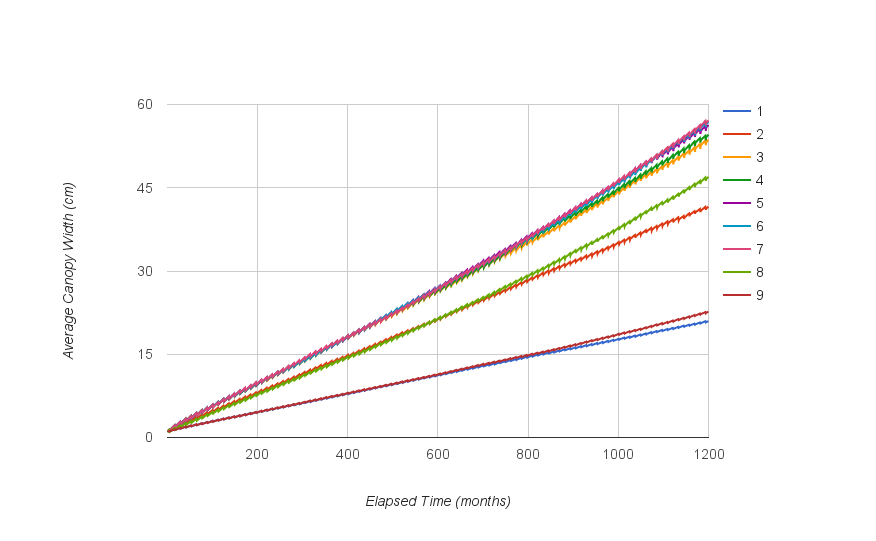
\includegraphics[width=\textwidth]{varying_resource_test.png}
	\caption{ Varying Resource Test: Average canopy width of a single plant throughout the simulations outlined in table \ref{tab:varying_resource_test_simulations}. }
	\label{fig:varying_resource_test}
\end{figure}

\subsubsection{Shade Test} \label{subsubsec:shade_test}

Plant's that are heavily dependent on illumination struggle to grow in areas shaded by the canopy of larger plants. To test this is modelled in the ecosystem simulator, a simulation is run with two species: \textit{S$_{smallroots}$} and grass (see appendix \ref{AppendixB} for specie details).  \textit{S$_{smallroots}$} is a custom specie created for the purpose of this test which has very small roots growth. This is important so as to focus on the effects of illumination and minimize the influence of drought. Figure \ref{fig:shade_test}, which illustrates the state of the simulation after fifty years, shows the grass struggling to grow in areas directly below the canopies of \textit{S$_{smallroots}$}.

\begin{figure}
\center
	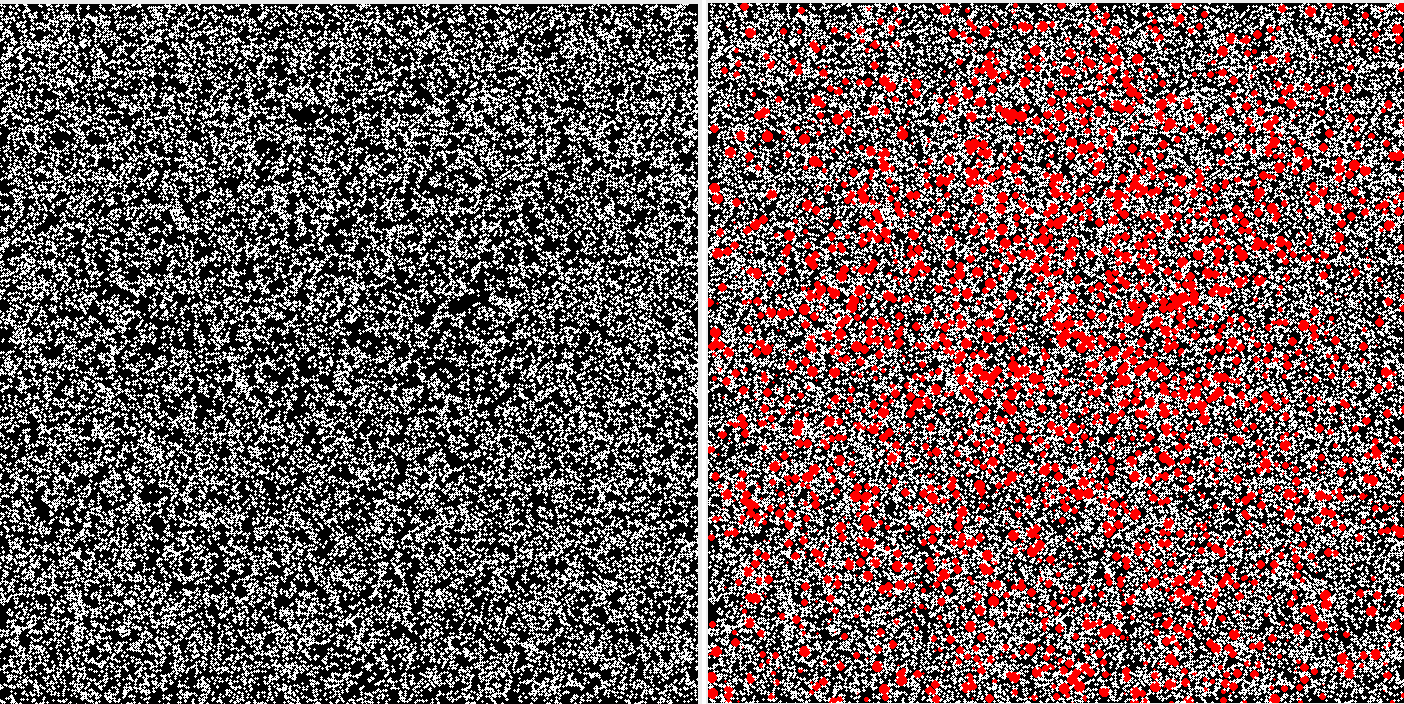
\includegraphics[width=\textwidth]{shade_propagation_test.png}
	\caption{ Shade Test: Simulation with \textit{S$_{smallroots}$} (red), grass (white) after fifty years. Left without rendering instances of \textit{S$_{smallroots}$} to visualise the effects of the shade}
	\label{fig:shade_test}
\end{figure}

\subsubsection{Shade-loving Test} \label{subsubsec:shade_loving_test}

Species which strive in shaded areas and struggle to survive in open spaces directly illuminated by the sun are deemed to be shade-loving. The shade can be caused by the terrain relief or by the shadow cast by the canopy of taller plants. To test whether the ecosystem simulator successfully caters for such plant species, a simulation is run identical to that done in the shade test (section \ref{subsubsec:shade_test}) but with shade-loving specie \textit{S$_{shadeloving}$} added (see appendix \ref{AppendixB} for specie details). As seen by the snapshot of the simulation after fifty years illustrated in figure .., instances of \textit{S$_{shadeloving}$} only appear in areas directly covered by the canopies of \textit{S$_{smallroots}$}.

\begin{figure}
\center
	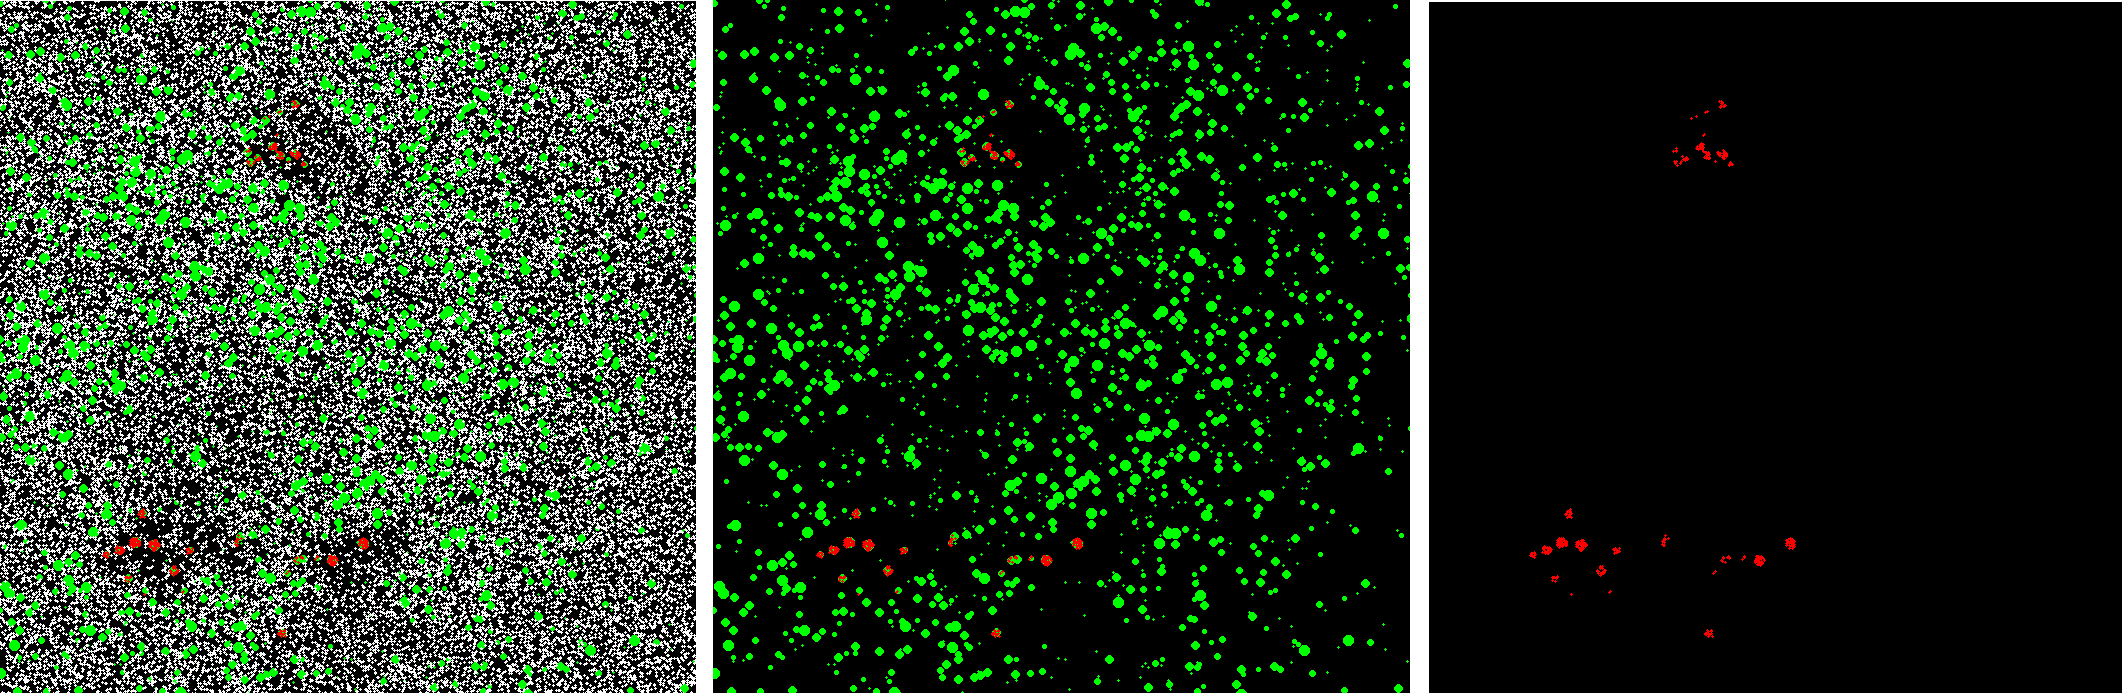
\includegraphics[width=\textwidth]{shade_loving_test.png}
	\caption{ Shade Loving Test: Simulation with \textit{S$_{smallroots}$} (green), grass (white) and \textit{S$_{shadeloving}$} after fifty years. From left-to-right: All species, excluding grass and only \textit{S$_{shadeloving}$}. As can be seen, \textit{S$_{shadeloving}$} strive under the canopies of \textit{S$_{smallroots}$}.}
	\label{fig:shade_loving_test}
\end{figure}
